\chapter{Experimental Methods} \label{chap:experimental-methods}
The following chapter presents the methods used for investigating the physical properties of semiconductor nanostructure specimens using off-axis electron holography, including their preparation, numerical modeling and the automation of the measurement and reconstruction process.
\section{Specimen Preparation} \label{sec:specimen-preparation}
Following the rapid development of integrated circuits (particularly in regards to their transistor density) in the 1980s and onwards, focused ion beam (FIB) milling has emerged as one of the most well established techniques for the analysis of such nanoscale structures \cite{Orloff2003,Giannuzzi2005}. Resembling a scanning electron microscopes (SEM), the FIB substitutes the focused electron beam with a focused ion beam produced by high electric fields \cite{Orloff2003,Giannuzzi2005}. While liquid metal ion sources (LIMS), especially Ga ion sources, comprise a large share of currently available instruments, gas field ion sources (GFIS) using plasma beams of noble gases, such as Xe, have become more widespread in recent time \cite{Orloff2003,Giannuzzi2005,Burnett2016}. The FIB's inherently destructive behavior towards the specimen by ion implantation into the specimen surface makes it a suitable tool for high precision milling \cite{Orloff2003,Giannuzzi2005}. This ability to remove selected areas with a precision of $\SI{10}{\nm}$ or less has established FIB milling as an viable and practical technique that goes far beyond TEM specimen preparation \cite{Orloff2003,Giannuzzi2005}.

The following \cref{ssec:specimen-preparation-capacitor,ssec:specimen-preparation-pn-junction} give a brief insight into the preparation of a coplanar capacitor and $p$-$p^+$-$n^+$-junction specimen using a FEI™ Helios NanoLab 600 DualBeam, consisting of both a SEM and a FIB.
\newpage
\subsection{Coplanar Capacitor} \label{ssec:specimen-preparation-capacitor}
The first specimen, a coplanar capacitor, is used a reference specimen for evaluation purposes due to its well known geometry, electric behavior and potential distribution.

The capacitor was produced utilizing FIB milling of an Au~film (roughly $\SI{25}{\um} \times \SI{16}{\um} \times \SI{3}{\um}$), which was transferred using an Oxford Instruments™ OmniProbe micromanipulator and contacted via FIB induced Pt~deposition onto a Protochips™ MEMS-based carrier FIB-E-Chip (\cref{fig:capacitor-specimen-FIB-preperation-SEM}a).
\begin{figure}[H]
	\centering
	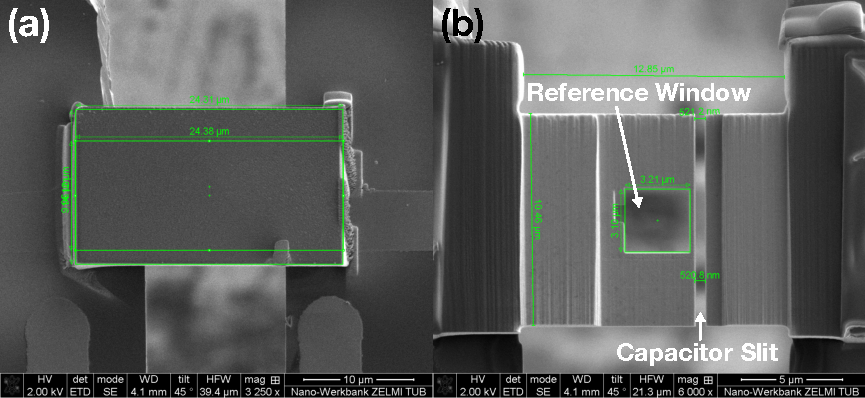
\includegraphics[width=\textwidth]{Figures/Specimen/Capacitor/capacitor-specimen-FIB-preperation-SEM.pdf}
	\caption{SEM images of the coplanar capacitor with (a) the placement/contacting (FIB induced Pt~deposition) of the Au~film and (b) the finished processed capacitor with a reference window in the left electrode.}
	\label{fig:capacitor-specimen-FIB-preperation-SEM}
\end{figure}
In the area of interest, the Au~film was thinned to a thickness of approximately $\SI{500}{\nm}$, separated over the entire width of the film (parallel to the electrodes of the carrier chip) to a distance of approximately $\SI{500}{\nm}$, resulting in two free-standing coplanar electrodes, and fitted with a reference window of roughly $\SI{3}{\um} \times \SI{3}{\um}$ near the slit of the capacitor (\cref{fig:capacitor-specimen-FIB-preperation-SEM}b). This cutout serves as an almost undisturbed region for the reference wave to propagate through, since the conductive edge of the reference window acts like a Faraday cage, therefore shielding the reference wave from unwanted modulations, which are especially present in electric biasing EH \cite{Wagner2019,Wagner2022}.
\newpage
\subsection[\texorpdfstring{$p$-$p^+$-$n^+$}{\textit{p}-\textit{p}\textsuperscript{+}-\textit{n}\textsuperscript{+}}-Junction]{$\boldsymbol{p}$-$\boldsymbol{p^+}$-$\boldsymbol{n^+}$-Junction} \label{ssec:specimen-preparation-pn-junction}
The second specimen, a $p$-$p^+$-$n^+$-junction, was cut out from a Si~wafer using standard FIB procedures and placed (similar to the above described coplanar capacitor) onto the carrier chip (\cref{fig:pn-junction-specimen-FIB-preperation-SEM}a and b).
\begin{figure}[H]
	\centering
	\includegraphics[width=\textwidth]{Figures/Specimen/pn-Junction/pn-junction-specimen-FIB-preperation-SEM.pdf}
	\caption{SEM images related to the specimen preparation of the $p$-$p^+$-$n^+$-junction with (a) the electrode geometry of the FIB-E-Chip, (b) the transfer of the FIB cut-out using the micromanipulator, (c) the contacted TEM lamella featuring the $p$-$p^+$-$n^+$-junction and a reference window close to it and (d) a side view of the TEM lamella during the thinning and cleaning process.}
	\label{fig:pn-junction-specimen-FIB-preperation-SEM}
\end{figure}
The lamella was contacted (FIB induced Pt~deposition) in such a way that the interface of the junction sits parallel to free-standing electrodes of the carrier chip (\cref{fig:pn-junction-specimen-FIB-preperation-SEM}c). The finished specimen was thinned to a thickness of approximately $\SI{350}{\nm}$ and fitted with a reference window close to the $p^+$-$n^+$-junction (\cref{fig:pn-junction-specimen-FIB-preperation-SEM}d). Through this geometry, the diode current is directly guided through the lamella (and its surface) with externally applied bias.
\newpage
\section{Numerical Modeling} \label{sec:numerical-modeling}
In order to accurately interpret and understand the experimental results obtained from off-axis electron holography measurements of the above mentioned two specimens, 2D~numerical simulations were carried out using different finite element method (FEM) software packages.
\subsection{2D Modeling of the Specimen} \label{ssec:2d-modeling-specimen}
A half-modeling approach that utilities the axial symmetry of the specimens can be used to reduce the computational complexity of the simulations. Specifically, only half of the specimens and stray fields were simulated, which significantly reduced the amount of RAM and computation time needed to obtain results. In order to obtain physical quantities, such as the electrostatic potential or phase, from the simulated half-model, appropriate adjustments were made to account for the symmetry of the problems.

The coplanar capacitor was modeled using the \emph{ONELAB} software bundle \cite{Geuzaine2013}, consisting of \emph{Gmsh} (a FEM mesh generator) \cite{Geuzaine2009} and \emph{GetDP} (a discrete physical problem solver) \cite{Dular1998}. For this, two coplanar plates of thickness $t = \SI{250}{\nm}$ each were placed $d = \SI{480}{\nm}$ apart from each other, with the stray field extending into the vacuum below the specimen, for a total dimension of $\SI{5000}{\nm} \times \SI{8000}{\nm}$ (\cref{fig:specimen-capacitor-layout}). The two capacitor plates were biased with $-U_{ext}$ and $U_{ext}$ using Dirichlet boundary conditions, whereas the vacuum uses a von~Neumann boundary condition of zero.
\begin{figure}[H]
	\centering
	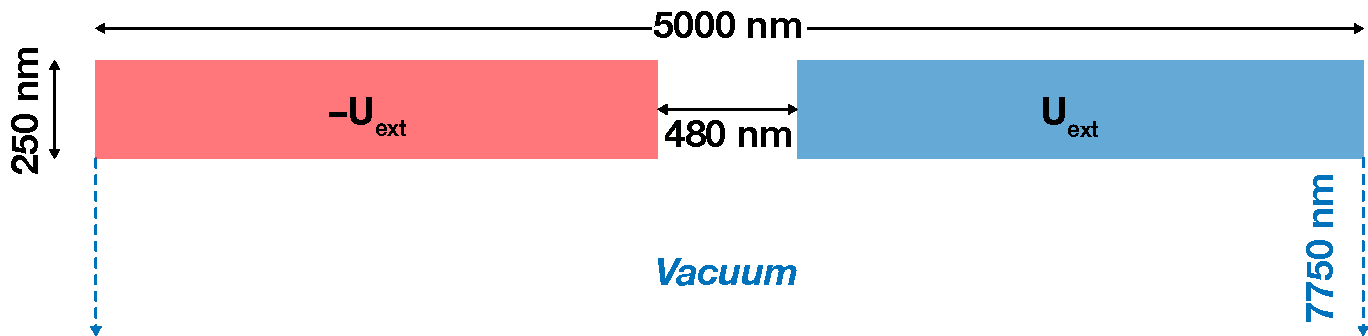
\includegraphics[width=\textwidth]{Figures/Specimen/Capacitor/specimen-capacitor-layout.pdf}
	\caption{Schematic illustration of the coplanar capacitor modeled using \emph{ONELAB}. The capacitor plates are spaced $d = \SI{480}{\nm}$ with a thickness of $t = \SI{250}{\nm}$ each, while the stray field extends into the vacuum region below the specimen for $\SI{7750}{\nm}$. Both capacitor plates are biased with $-U_{ext}$ and $U_{ext}$ using Dirichlet boundary conditions, whereas the vacuum uses a von~Neumann boundary condition of zero.}
	\label{fig:specimen-capacitor-layout}
\end{figure}
The $p$-$p^+$-$n^+$-junction was modeled using \emph{nextnano}. Here, three different Si~specimen regions with two different doping concentrations and equivalent lengths of $\SI{1000}{\nm}$ and thicknesses of $\SI{150}{\nm}$ each were defined (\cref{fig:specimen-nextnano-layout}). The weakly doped ($\SI[per-mode=power]{1e16}{\per\cubic\cm}$) $p$-region on the left features an abrupt transition to a heavily doped ($\SI[per-mode=power]{1e19}{\per\cubic\cm}$) $p^+$-region on the right, which in turn features an abrupt transition to an equivalently doped $n^+$-region. The specimen is further equipped with Schottky Pt contacts of $\SI{50}{\nm}$ width on both sides. The stray field extends below the specimen into the vacuum region for $\SI{2500}{\nm}$, while a temperature of $T = \SI{300}{\kelvin}$ was assumed.

To reduce the already high computational cost of the \emph{nextnano} simulation, the 2D~grid points were spaced only in the regions of interest (i.\,e.\ the $p$-$p^+$ and $p^+$-$n^+$-junction) with a distance of $\SI{1}{\nm}$. For the rest of the specimen and vacuum region, a grid point spacing of $\SI{10}{\nm}$ is sufficient, with no abrupt transition between the two spacing factors.
\begin{figure}[H]
	\centering
	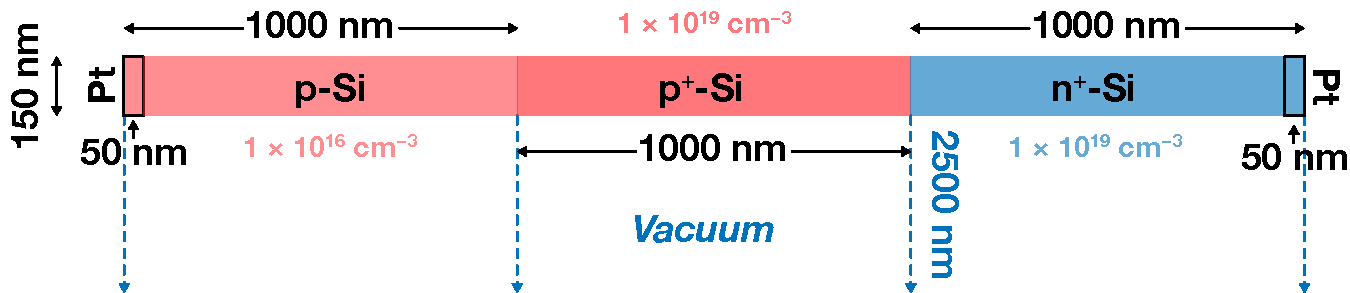
\includegraphics[width=\textwidth]{Figures/Specimen/pn-Junction/specimen-nextnano-layout.pdf}
	\caption{Schematic illustration of the $p$-$n$-junction modeled using \emph{nextnano}. All three specimen regions feature the same width of $\SI{1000}{\nm}$ and thickness of $\SI{150}{\nm}$ each, while the doping abruptly changes from $\SI[per-mode=power]{1e16}{\per\cubic\cm}$ to $\SI[per-mode=power]{1e19}{\per\cubic\cm}$ at the $p$-$p^+$-junction. Furthermore, Pt contacts are placed at both ends of the same with a width of $\SI{50}{\nm}$ each, whereas the stray field extends into the vacuum region for $\SI{7750}{\nm}$.}
	\label{fig:specimen-nextnano-layout}
\end{figure}
The coupled Schrödinger-Poisson-current equations were then solved iteratively, with the maximum number of iterations limited to $\num{10000}$.
\subsection{Simulated Potential and Phase} \label{ssec:FEM-simulated-potential-and-phase}
In order to extract the electrostatic potential, and with that the electric phase, from the above mentioned 2D~simulations, the output has to be parsed differently, depending on which software package was used.

For the \emph{ONELAB} simulation, the output of the simulation is the electrostatic potential with regards to the generated mesh of the corresponding physical problem. These mesh-based values can be exported to a generic text file using the \emph{CutParametric} plugin, where the required computation time and storage is heavily dependent on the global mesh size factor and number of points used for the parametric plane. This generic text file can then be parsed to \textsc{python}, where the electrostatic potential values are contained in the last 1D~column and reshaped to a proper 2D~grid according to the previously defined dimensions of the simulation. The object phase $\varphi_{\mathit{obj}}$ can be obtained by projecting the electrostatic potential in the electron beam propagation direction, i.\,e.\ by calculating the cumulative sum over all columns and extracting the last row. In addition, similar to the experimental measurement, a reference phase $\varphi_{\mathit{ref}}$ of the same width but different position can be subtracted from the object phase between the capacitor plates. Furthermore, the different contributions to the calculated phase $\varphi = \varphi_{\mathit{obj}} - \varphi_{\mathit{ref}}$ from the capacitor itself and the stray field can be adjusted through a pair of weighted thickness parameters influencing the projection of the electrostatic potential. At last, the calculated phase is multiplied with the interaction constant $\sigma$ (\cref{eq:electron-holography-electrostatic-potential}), where $\sigma = \SI{6.53}{rad \per \volt \um}$ for an acceleration voltage of $U_{\mathit{acc}} = \SI{300}{\kilo\volt}$ \cite{Beleggia2014}.

In comparison, \emph{nextnano} outputs the calculated electrostatic potential using the \emph{Visualization Toolkit} (i.\,e.\ \texttt{.vtr}) file format. Here, the \emph{nextnanopy} software package \cite{nextnanopy} provides an easy-to-use interface for parsing \emph{nextnano}'s output, where, in addition to the electrostatic potential, the Euclidian coordinates of the simulated grid points, along with their corresponding units, can be accessed. Similar to above, the object phase $\varphi_{\mathit{obj}}$ is calculated from the projection of the electrostatic potential through a cumulative sum over all columns (\cref{fig:flowchart-automatic-nextnano-post-processing}).
\begin{figure}[H]
	\centering
	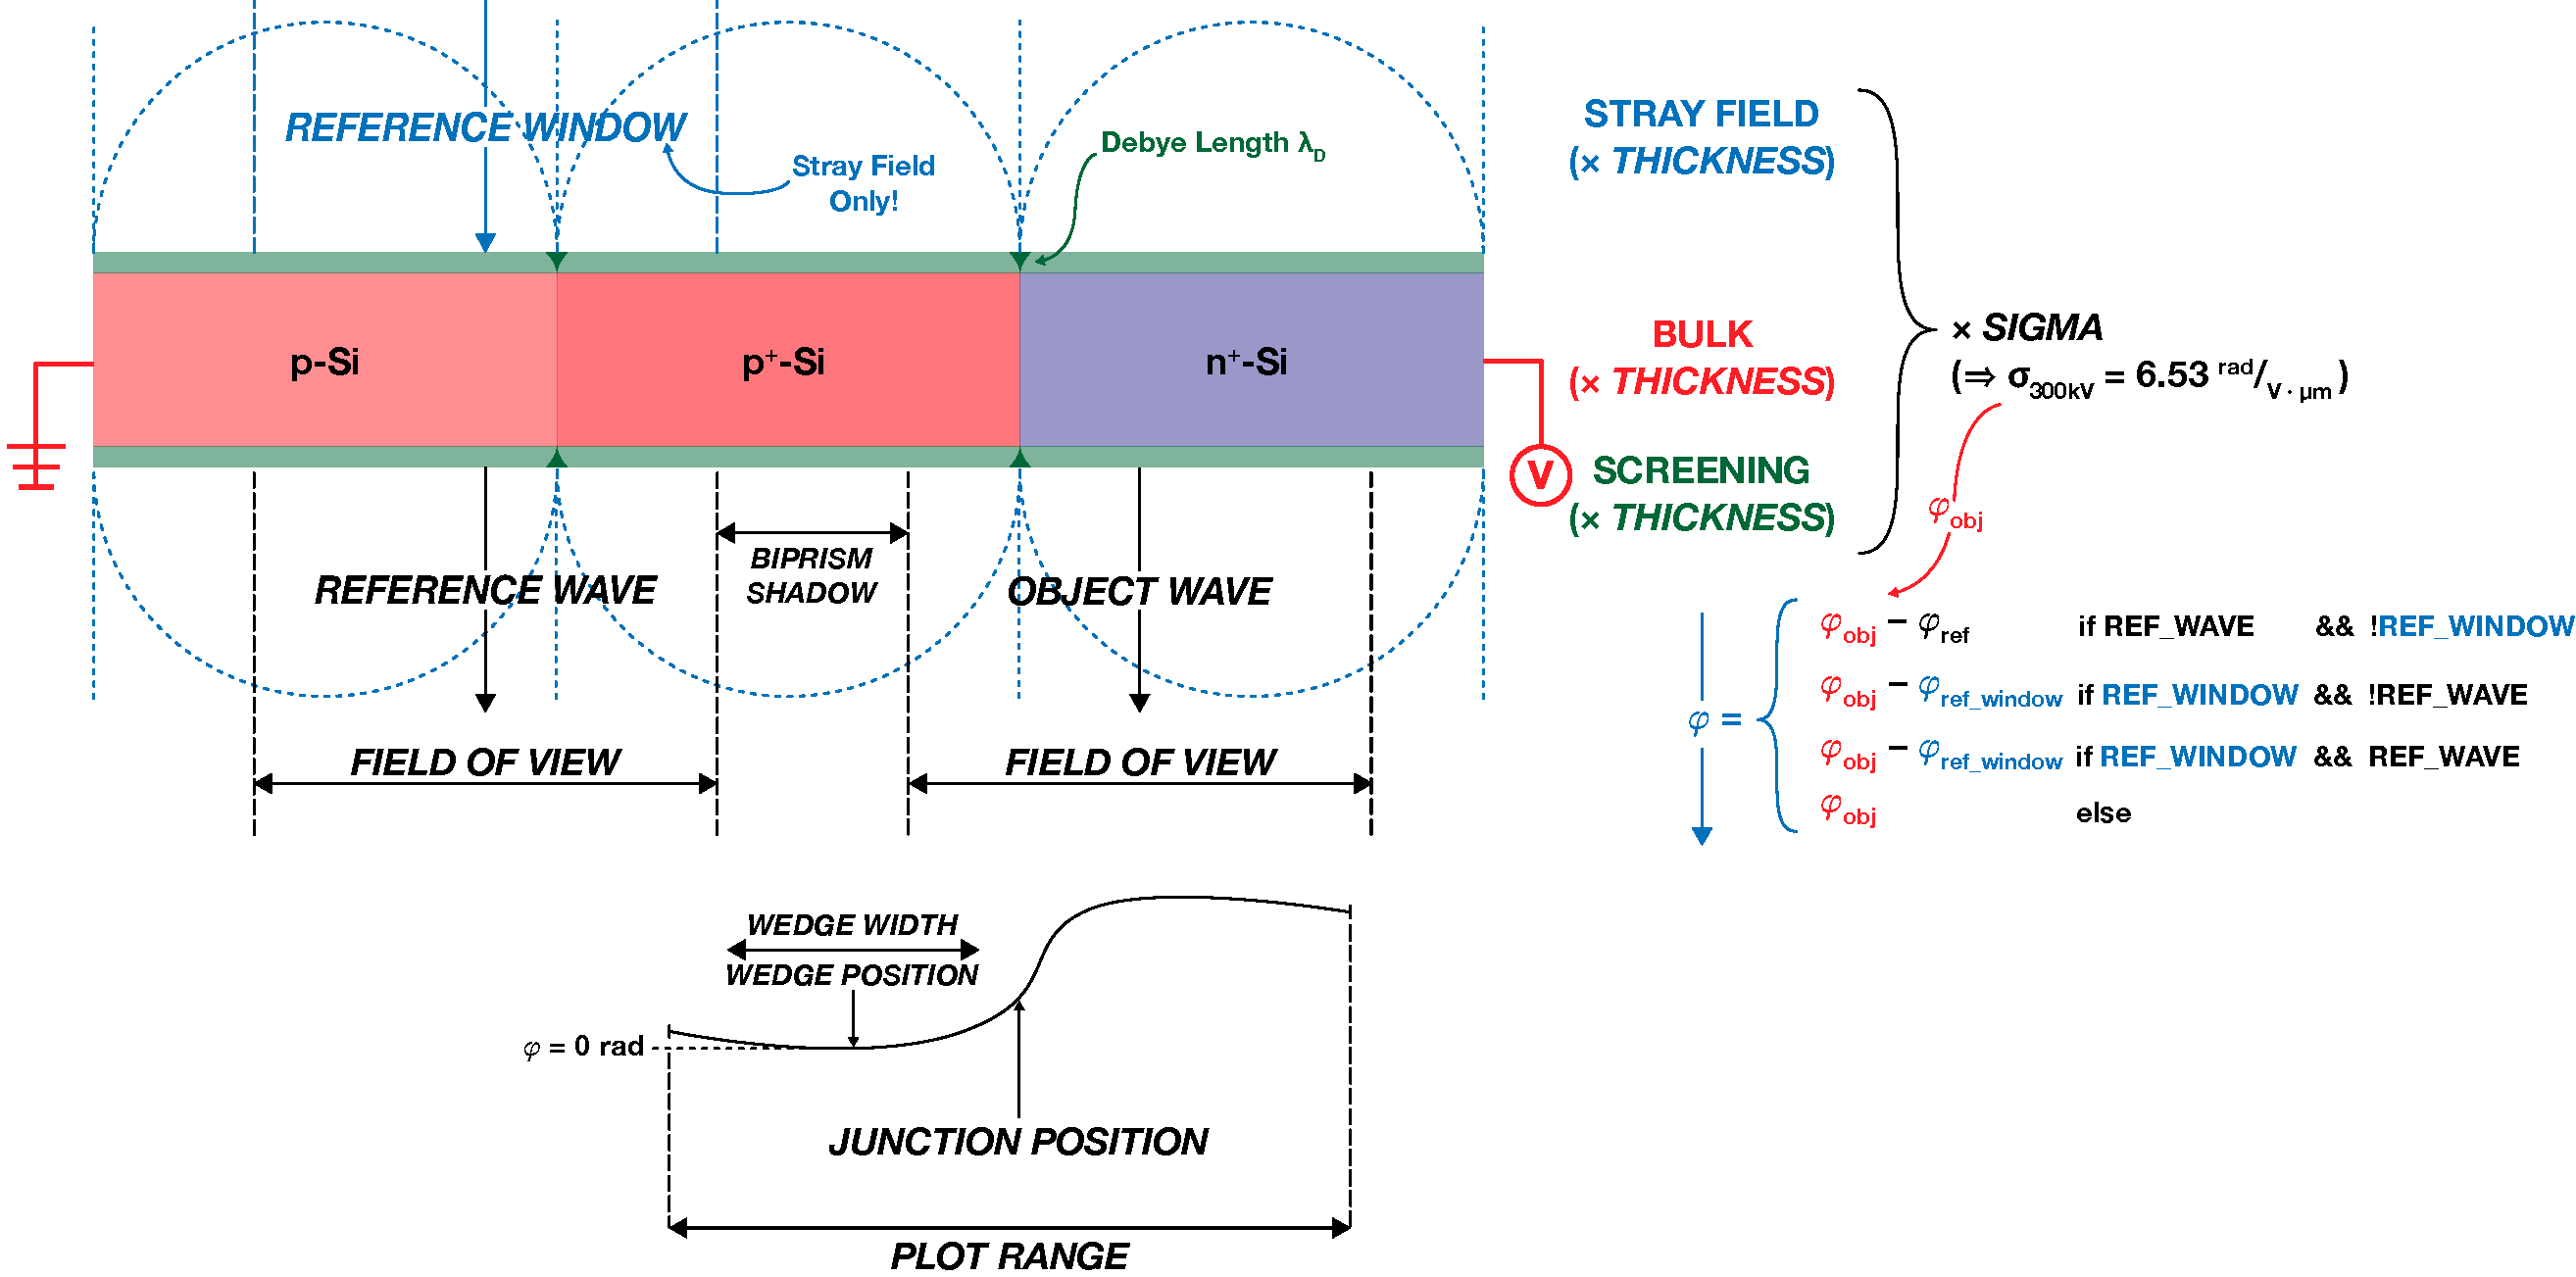
\includegraphics[width=\textwidth]{Figures/Schematics/Automation/flowchart-automatic-nextnano-post-processing.pdf}
	\caption{Schematic illustration detailing how the phase is calculated from the simulated electrostatic potential using \emph{nextnano} and \emph{nextnanopy}. Here, the object wave and reference wave strech over the same field of view and are separated by the biprism shadow. Either the reference phase $\varphi_{\mathit{ref}}$ or the reference window phase $\varphi_{\mathit{ref\_window}}$, which only contains contributions from the stray field, is subtracted from the object phase $\varphi_{\mathit{phase}}$, resulting in $\varphi$.}
	\label{fig:flowchart-automatic-nextnano-post-processing}
\end{figure}
Here, the object wave and reference wave are separated by the biprism shadow, and the width of each wave is given by the field of view. In contrast to the above described coplanar capacitor, the phase is not only made up of contributions from the inner bulk-like material and the stray field, but also a surface layer, where all three contributions can again be adjusted through a set of weighted thickness parameters. An additional reference window contribution $\varphi_{\mathit{ref\_window}}$ is added, which is equal to only the stray field contribution inside the reference wave region. Depending on the choice of parameters, the resulting phase $\varphi$ is calculated through the difference of the object phase $\varphi_{\mathit{obj}}$, which contains the acceleration dependent interaction constant $\sigma$ (\cref{eq:electron-holography-electrostatic-potential}), with either the reference phase $\varphi_{\mathit{ref}}$ or the reference window phase $\varphi_{\mathit{ref\_window}}$.
\newpage
\section{Off-Axis Electron Holography}
In order to investigate the two above detailed specimens, a self-developed and extensive automation scheme for the measurement and reconstruction of off-axis EH is utilized.
\subsection{Experimental Setup} \label{ssec:off-axis-EH-experimental-setup}
The electron holographic investigations were conducted on the FEI™ Titan 80-300 Berlin Holography Special TEM at an acceleration voltage of $U_{\mathit{acc}} = \SI{300}{\kilo\volt}$. Furthermore, the TEM was used in Lorentz mode for medium resolution, yielding a field of view of approximately $\SI{1.5}{\um} \times \SI{1.5}{\um}$. The biprism was oriented parallel to the slit of the capacitor and the interface of the $p^+$-$n^+$-junction such that reference wave was taken from an area within the reference window (\cref{fig:TEM-overview-holo-BP}).
\begin{figure}[H]
	\centering
	\includegraphics[width=\textwidth]{Figures/Specimen/TEM-overview-holo-BP.pdf}
	\caption{TEM overview micrographs of (a) the coplanar capacitor and (b) the $p$-$p^+$-$n^+$-junction, both acquired in Lorentz mode (i.\,e.\ with the objective lens disabled) and with the biprism and reference window visible. Here, the filament voltage $U_f$ is turned off (i.\,e.\ $U_f = \SI{0}{\volt}$) for (a) and at $U_f = \SI{60}{\volt}$ for (b).}
	\label{fig:TEM-overview-holo-BP}
\end{figure}
Here, the filament voltage was adjusted to accommodate hologram widths between $\SI{1}{\um}$ and $\SI{1.5}{\um}$. The external bias was applied via a Keithley™ 2460 Source Measure Unit (SMU), connected to a modified Protochips™ Aduro electrical biasing TEM holder \cite{Wagner2022}. Additionally, a Gatan™ US1000 CCD camera was used for the acquisition of the holograms.
\subsection{Automated Measurement} \label{ssec:holosuite-automated-measurement}
Modern-day science, with its ever-increasing datasets \cite{Tate2016,Baldwin2018,Ophus2019,Spurgeon2021}, benefits greatly from automated and integrated workflows. Automation not only results in significant time savings, allowing scientists to better allocate their time towards further research, but it also prevents (sometimes difficult to detect) human errors caused by the repetition of mundane tasks. For this reason, extensive automation routines (named \emph{HoloSuite}) have been developed to deal not only with the actual measurements, but also with the reconstruction and post-processing of off-axis electron holograms.

Using the experimental setup detailed in the previous \cref{ssec:off-axis-EH-experimental-setup}, the automated measurement implemented in \emph{HoloSuite} can be broken down into three main sections (\cref{fig:flowchart-automatic-holography-measurement}): To begin with, the first section acquires the desired number of holograms at the specified external biasing voltages, along with their normalization holograms and $I$-$V$~curves, followed by the second section, which repeats this hologram acquisition with the specimen removed, after which the third section measures the dark currents with the electron beam blanked.
\begin{figure}[H]
	\centering
	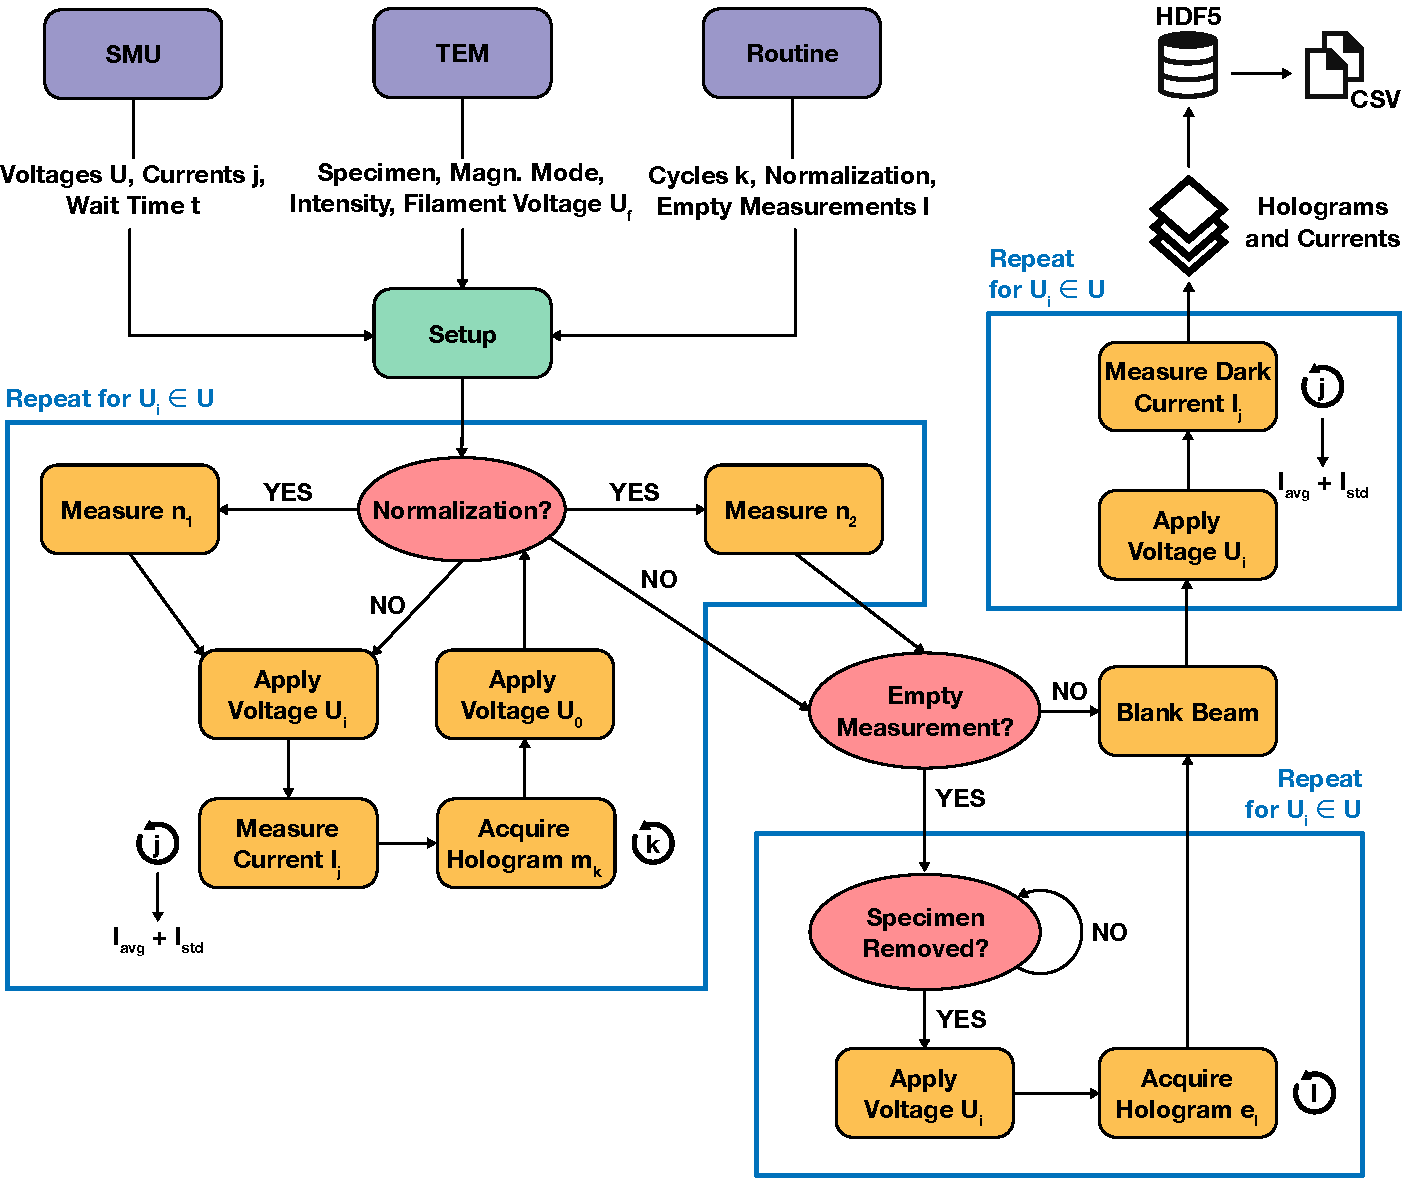
\includegraphics[width=\textwidth]{Figures/Schematics/Automation/flowchart-automatic-holography-measurement.pdf}
	\caption{Flowchart detailing the automated measurement process using the self-developed \emph{HoloSuite} software package: Extensive customization options regarding the various measurement parameters concerning the SMU, TEM and measurement routine allow for the fully automated acquisition of the electron holograms $m_k$, the normalization holograms $n_1$ and $n_2$, and the empty holograms $e_l$ for every applied bias voltage $U_i$, as well as the average (dark) currents $I_{\mathit{avg}}$ and corresponding standard deviation $I_{\mathit{std}}$.}
	\label{fig:flowchart-automatic-holography-measurement}
\end{figure}
In order to obtain the desired measurement data, \emph{HoloSuite} offers extensive customization options regarding the various measurement parameters found in a modern experimental setup. These parameters can be classified into three groups, depending on whether they concern the SMU, the TEM or the actual measurement routine. The parameters regarding the SMU specify the external biasing voltages $U_{\mathit{ext}}$ that are applied to the specimen, defined by a start and end voltage, along with the step size between them, the voltage and current range of the SMU, the number of currents $j$ that are measured for each applied voltage $U_i$ and subsequently averaged, and the wait time $t$ between the various changes of the SMU and the hologram acquisition. The second set of parameters concerns all settings regarding the TEM and is mostly used to properly name the resulting dataset, containing the name of the specimen, the magnification mode (i.\,e.\ SA or Lorentz mode), the C2~lens intensity, the filament voltage $U_f$ and the acceleration voltage $U_{\mathit{acc}}$, along with the exposure time $t_{\mathit{exp}}$ for each acquired hologram. The final set of parameters deals with the automated measurement routine itself and contains the number of holograms $k$ acquired per applied voltage $U_i$, whether to obtain two normalization holograms $n_1$ and $n_2$ and the number of empty holograms $l$ per applied voltage $U_i$.

With the all required parameters specified, \emph{HoloSuite} first connects to the SMU using a network socket and a specified IP~address and port. If the connection was successful, the output terminals of the SMU are turned on and the specified voltage and current ranges are applied (therefore disabling the default auto range option). The remote connection to the TEM is likewise established using the \emph{temscript} software package, a \textsc{python} wrapper for the TEMScripting interface by FEI™ \cite{temscript}, via a provided IP~address and port. After a successful connection to the TEM, the output dataset is allocated on the hard disk, where the filename is generated from the second set of parameters specified above. The dataset itself is written to and accessed by using the \emph{h5py} package, where the open HDF5 standard is optimized for storing and accessing large amounts of data and not only allows filesystem-like arbitrary organization into (sub-)groups, but also flexible metadata associated with every object \cite{Collette2014}.

The first series of measurements is acquired by looping over every external bias voltage, starting from the one with the smallest absolute value\footnote{Usually $U_{\mathit{ext}} = \SI{0}{\volt}$.} and increasing in an alternating pattern between forward and reverse bias\footnote{This is done in order to minimize the change of damaging the specimen by suddenly applying a large external bias voltage.}. For every voltage $U_i$, a corresponding group is created in the HDF5 dataset, with the applied voltage as its name. After which, if specified, the first normalization hologram $n_1$ of the unbiased specimen (i.\,e.\ $U_{\mathit{ext}} = \SI{0}{\volt}$), with the desired exposure time $t_{\mathit{exp}}$, is acquired. Afterwards, the current biasing voltage $U_i$ is applied via the SMU and the current is measured $j$ times, yielding the corresponding average current $I_{\mathit{avg}}$ and standard deviation $I_{\mathit{std}}$. Thereafter, the $k$ actual electron holograms $m_k$ are measured, each with an exposure time of $t_{\mathit{exp}}$. Upon applying a biasing voltage of $U_{\mathit{ext}} = \SI{0}{\volt}$ again, the second normalization hologram $n_2$ is acquired, if specified.

The second series of measurements contains all empty holograms, where $l$ empty holograms $e_l$ are acquired for every applied voltage $U_i$. Here, if needed, the user is given the opportunity to remove the specimen from the field of view and thus also from acquired holograms.
\newpage
Regardless of whether \emph{HoloSuite} is set to acquire empty holograms or not, the automated measurement always contains a series of dark currents. Here, the electron beam is first blanked, after which the current is measured $j$ times for every applied voltage $U_i$, resulting in the corresponding average dark current $I_{\mathit{avg}}$ and standard deviation $I_{\mathit{std}}$.

In addition to the HDF5 dataset, that not only contains all holograms but also the average (dark) currents $I_{\mathit{avg}}$ and corresponding standard deviations $I_{\mathit{std}}$, the $I$-$V$~curves are written as comma-separated values (CSV) to a text file. \emph{HoloSuite} therefore significantly cuts down on measurement time, reducing the required time (excluding TEM alignment) from a full work day to around 30~minutes or less, where the resulting HDF5 dataset ranges from a few hundred~MB to multiple~GB, depending on the specified voltage range and desired number of holograms. The automated measurement finishes by unblanking the electron beam, turning off the SMU outputs and closing the connecting network socket.
\subsection{Automated Reconstruction} \label{ssec:holosuite-automated-reconstruction}
In order to obtain the full set of information carried by the previously acquired electron
holograms, a two-step reconstruction process has to be carried out \cite{Voelkl1999,Lehmann2002,Lichte2008}. While improving the signal-to-noise ratio (SNR) can, in principle, be done by lengthened exposure times $t_{\mathit{exp}}$, a multitude of instrumental instabilities (especially in the high-resolution domain) make this approach, at least without sophisticated feedback control in the experimental setup \cite{Gatel2018,Takahashi2020}, practically unfeasible \cite{Niermann2014}. Using a special reconstruction algorithm featuring an advanced averaging scheme implemented in the \emph{holoaverage} software package proves to be a viable and suitable solution \cite{Niermann2014}, motivating the acquisition of multiple holograms per applied bias voltage $U_i$ in the automated measurement process of \emph{HoloSuite}.
\newpage
With the measurement dataset obtained by automated acquisition detailed in \cref{ssec:holosuite-automated-measurement}, the automated reconstruction and post-processing of electron holograms implemented in \emph{HoloSuite} can be divided into two parts (\cref{fig:flowchart-automatic-holography-post-processing}): While the first part deals with the actual reconstruction of the electron holograms using \emph{holoaverage}'s averaging scheme \cite{Niermann2014}, the second part obtains various physical quantities of the specimen, such as the phase modulation $\varphi$ and its first- and second-order derivative $\dv*{\varphi}{x}$ and $\dv*[2]{\varphi}{x}$ (which are proportional to the electric field $E$ and the charge carrier density $\rho$, respectively), through a multi-step post-processing method.
\begin{figure}[H]
	\centering
	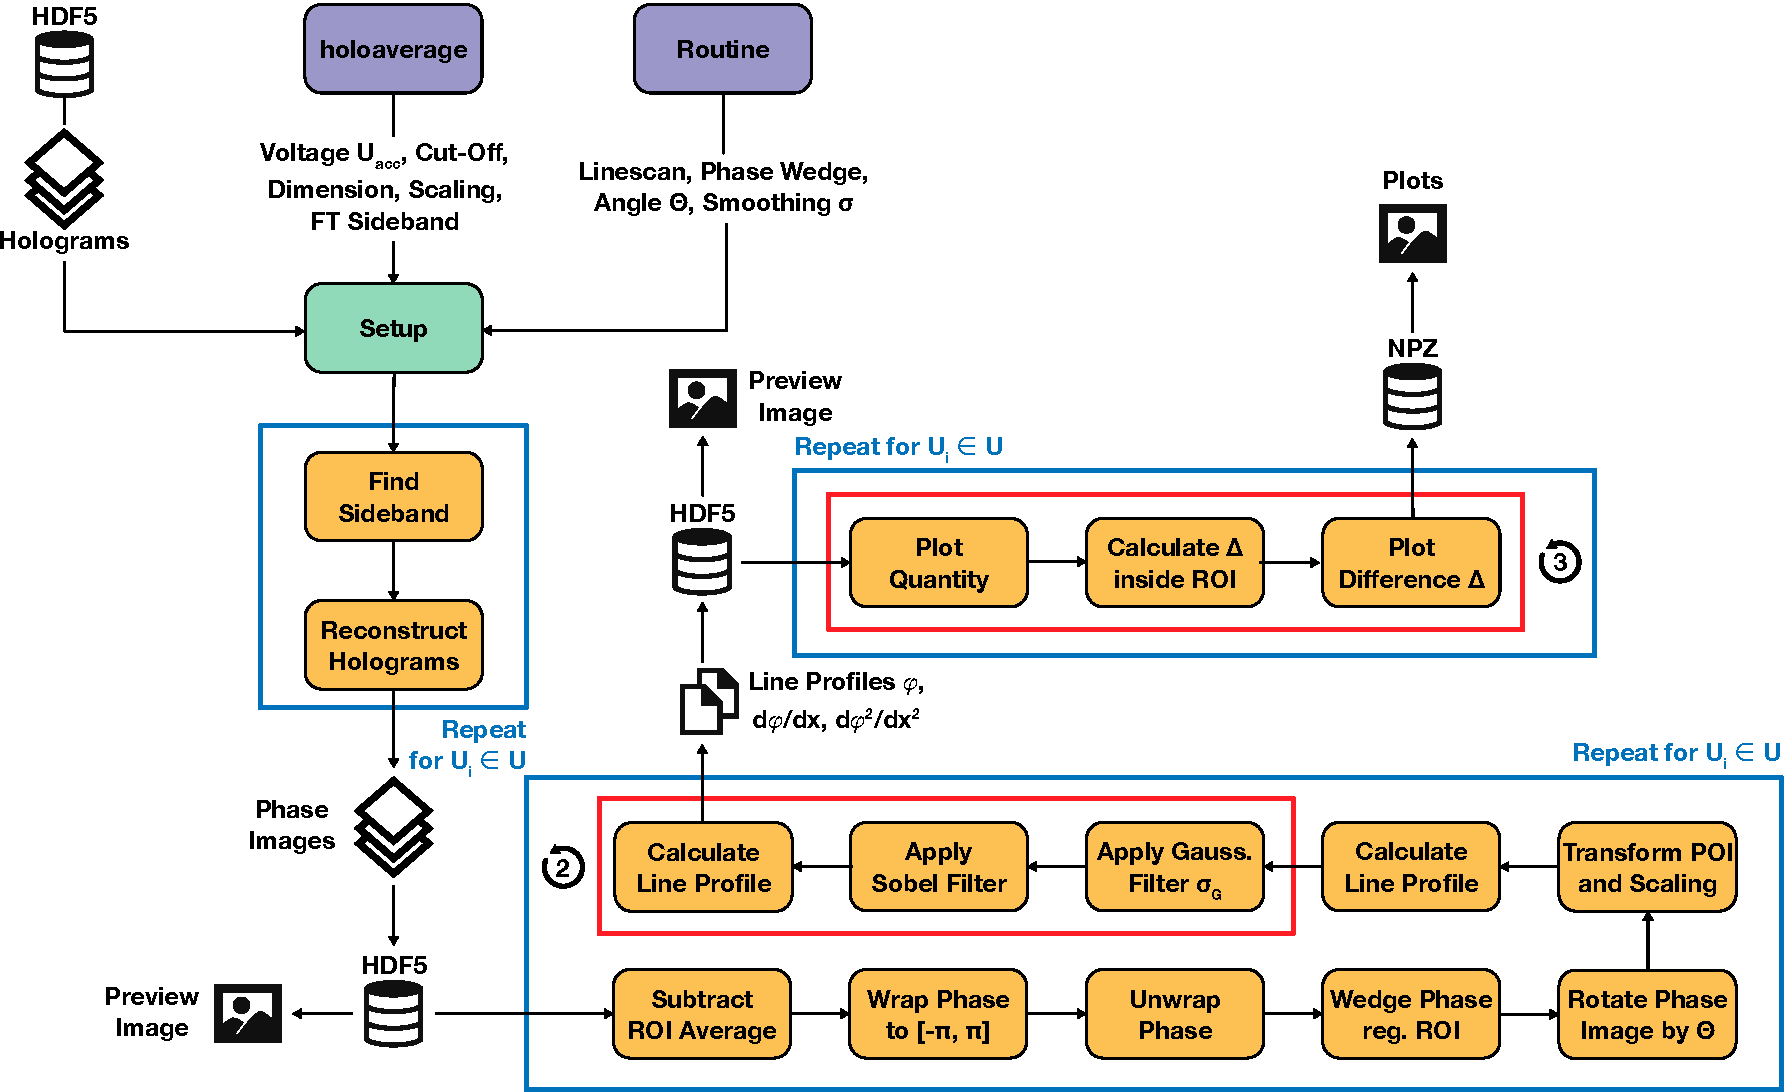
\includegraphics[width=\textwidth]{Figures/Schematics/Automation/flowchart-automatic-holography-post-processing.pdf}
	\caption{Flowchart detailing the automated reconstruction and post-processing method using the self-developed \emph{HoloSuite} software package: Initially, the previously acquired electron holograms are reconstructed using \emph{holoaverage}'s reconstruction algorithm \cite{Niermann2014}, followed by a multi-step post processing method to obtain various physical quantities of the specimen, such as the phase modulation $\varphi$ and its first- and second-order derivative $\dv*{\varphi}{x} \propto E$ and $\dv*[2]{\varphi}{x} \propto \rho$.}
	\label{fig:flowchart-automatic-holography-post-processing}
	\vspace*{-3mm}
\end{figure}
In line with the previously described automated measurement process, \emph{HoloSuite} offers extensive customization options regarding the actual electron hologram reconstruction as well as the post-processing routine. These parameters can again be classified into different groups, depending on whether they concern the electron hologram reconstruction using \emph{holoaverage} or the post-processing of these reconstructed holograms. The parameters regarding \emph{holoaverage} specify the acceleration voltage $U_{\mathit{acc}}$ used for acquisition, the cut-off frequency in Fourier space, the size of the reconstructed object hologram, the sampling factor and the quadrant of the sideband in Fourier space. The second set of parameters contains all the information needed for the post-processing of the reconstructed electron holograms, consisting of the line profile coordinates and width, the phase wedge position, width and number of times it is applied, the angle $\theta$ by which the electron holograms are rotated and the standard deviation $\sigma_G$ of the Gaussian kernel used for smoothing.

After all necessary parameters are specified, \emph{HoloSuite} begins with the reconstruction of the electron holograms through the supplied HDF5 dataset. For each applied bias voltage $U_i$, \emph{HoloSuite} automatically finds the pixel position of the sideband in Fourier space needed for reconstruction. This is done by cropping the electron holograms to the specified quadrant, on top of a (customize) cut-off around the edges\footnote{This additional cut-off around the edges of the isolated quadrant in Fourier space is done in order to ensure that the brightest pixel actually corresponds to the sideband and not the autocorrelation of the electron hologram.}, and finding the brightest pixel. After which, a (customizable) region of interest (ROI) around this pixel is isolated and a center of mass calculation is applied using the \emph{SciPy} software package \cite{Virtanen2020} (which is also used for the Fourier transform and the later image rotation, smoothing and derivative) to find the sub-pixel position of the sideband. This sub-pixel position of the sideband, along with all the above mentioned parameters, are passed to \emph{holoaverage}, yielding the (complex valued) averaged reconstructions of the normalized and drift aligned object holograms for every applied bias voltage $U_i$. In order to also obtain the phase images, the counterclockwise angles from the positive real axis on the complex plane are calculated using the \emph{NumPy} software package \cite{Harris2020} (which is also used for all general mathematical calculation, such as averaging, standard deviation and so forth). If specified, the two normalization measurements $n_1$ and $n_2$ are passed as pseudo-empty measurements to \emph{holoaverage} instead of the acquired holograms $e_l$.

After all acquired measurements have been reconstructed, \emph{HoloSuite} outputs all electron holograms and phase images to a HDF5 dataset, where each group corresponds to the applied bias voltage $U_i$ and contains two 2D~datasets with the above specified output dimension, along with one preview phase image (for a customizable bias voltage) as a TIFF file. In addition, all metadata provided by \emph{holoaverage}, such as the scaling factor of the reconstructed electron holograms and the spatial frequency of the reconstructed sideband, is copied over and written as attributes to the HDF5 output file for each dataset.

With the reconstruction completed, the phase images have to be post-processed using a comprehensive workflow. For this, \emph{HoloSuite} starts by looping over every phase image in the provided HDF5 dataset and subtracting the average of the phase wedge ROI (i.\, e. offsetting them so that they are close to zero within the phase wedge ROI). Since this leads to the phase images no longer being constrained to an interval of $\interval{-\pi}{\pi}$, they are again wrapped back to $\interval{-\pi}{\pi}$:
\begin{equation}
\vb*{\varphi}_{2\pi} = \arg\left(e^{i \cdot \vb*{\varphi}_{\mathit{off}}}\right),
\end{equation}
where $\vb*{\varphi}_{2\pi}$ represents the $\interval{-\pi}{\pi}$ wrapped phase image, $\vb*{\varphi}_{\mathit{off}}$ the non-constrained phase image obtained through the subtraction of the phase wedge ROI and $\arg$ the angle of the complex argument. This phase wrapping to $\interval{-\pi}{\pi}$ is done to ensure that the subsequent phase unwrapping using \emph{scikit-image}'s implementation \cite{Vanderwalt2014} of a fast 2D~and 3D~algorithm based on sorting by reliability following a non-continuous path \cite{Herraez2002,AbdulRahman2005} produces reliable results. After unwrapping, the average of the phase wedge ROI is again subtracted from the phase images. Next, the phase images are modulated using a self-developed phase wedge method, where for every row inside the phase wedge ROI, a linear fit is calculated. These multiple linear fits are then averaged, and this average linear fit is extrapolated to all rows of the phase image and subsequently subtracted. This procedure is then repeated for every column, resulting in the wedged phase image:
\begin{gather}
\vb*{\varphi}_w = \vb*{\varphi}_{\gamma} - \overline{\mathcal{X}}_R\left(\vb*{\varphi}_{\gamma}\right) - \overline{\mathcal{X}}_C\left(\vb*{\varphi}_{\gamma}\right), \label{eq:holosuite-phase-wedge} \\
\overline{\mathcal{X}}_R = \sum\limits_{a=1}^{p \in \mathbb{N}} \frac{\mathcal{X}\left(\vb*{\varphi}_{\gamma}^a\right)}{p} \quad ; \quad \overline{\mathcal{X}}_C = \sum\limits_{b=1}^{p \in \mathbb{N}} \frac{\mathcal{X}\left(\vb*{\varphi}_{\gamma}^b\right)}{p}, \label{eq:holosuite-phase-wedge-average-fit}
\end{gather}
with the wedged phase image $\vb*{\varphi}_w$, the unwrapped and phase wedge ROI average subtracted phase image $\vb*{\varphi}_{\gamma}$, the linear fit $\mathcal{X}$ applied to every row $a$ and column $b$ across the phase wedge width $p$ (with $a, b, p \in \mathbb{N}$), and the averaged linear fits $\overline{\mathcal{X}}_R$ and $\overline{\mathcal{X}}_C$. Since the averaged linear fits inside the phase wedge ROI are sometimes not sufficiently flat enough after one calculation, the phase wedge is applied multiple times, where the number of repetitions is customizable.

Next, the phase images are rotated by the specified angle $\theta$, where $\theta$ is chosen such that the $p$-$n$-junction is orthogonal to the $x$-axis. Rotating an image by $\theta \in \left\{n \cdot \pi / 2 \, \middle| \, n \in \mathbb{N}\right\}$ yields an output image of equal shape. If, however, the angle is chosen such that $\theta \in \mathbb{R} \setminus \left\{n \cdot \pi / 2 \, \middle| \, n \in \mathbb{N}\right\}$, the output image has to either be cropped (if the same shape as the input image is desired, therefore losing information) or reshaped (if the input image is to be completely contained within output image, therefore increasing the image's shape through interpolation). Here, the output image is reshaped, meaning that all spatially dependent parameters, such as the line profile position, the phase wedge position or the scaling factor, have to be recalculated through a transformation from the input image to the output image.

Following the rotation of the phase images and the transformation of all points of interests, the first set of line profiles is calculated using \emph{scikit-image} at the specified start and end point. For every phase image, the line profile is reduced across the specified line profile width from a 2D~rectangle to 1D~curve, where the aggregation of pixel values perpendicular to the line profile is calculated through averaging. This 1D line profile returns the phases $\varphi$ (i.\,e.\ the projected electrostatic potentials $\phi$) for every applied bias voltage $U_i$. In order to obtain a quantity proportional to the electric fields $E$ across the same line profile region, the first-order derivative in $x$-direction for all phase images is calculated. This is done through the convolution with a Sobel filter, where all phase images are smoothed beforehand using a 2D~Gaussian filter and the specified $\sigma_G$. After which, the same 1D line profile can be calculated, yielding $\dv*{\varphi}{x} \propto E$. A second subsequent and identical smoothing and second-order derivative is applied, from which, with the use of the aforementioned line profile, a quantity proportional to the charge carrier density $\rho$ can be calculated, resulting in $\dv*[2]{\varphi}{x} \propto \rho$. As with the automatic reconstruction using \emph{holoaverage}, a preview PNG image is saved for a customizable external bias voltage, with the phase wedge ROI and line profile area indicated by differently colored rectangles.

One of the advantages of the automated acquisition of large datasets is the ability to investigate the changes in the various physical properties of the specimen caused by applying an external bias voltage. Of particularly great interest is the change in the phase, and thus the first- and second-order derivative, when an external bias voltage is applied in both forward and reverse direction, compared to the case where no external bias voltage is applied. For the three above mentioned physical properties $\varphi$, $\dv*{\varphi}{x}$ and $\dv*[2]{\varphi}{x}$, this is done by:
\begin{itemize}
	\item \textbf{Phase $\varphi$}: Find the $\SI{10}{\percent}$ interval with the highest average value in a range of $\SIrange{40}{80}{\percent}$ and subtract if from the closest average to zero in a range of $\SIrange{10}{40}{\percent}$;
	\item \textbf{First-Order Derivative $\dv*{\varphi}{x} \propto E$}: Find the $\SI{10}{\percent}$ interval with the lowest average value in a range of $\SIrange{20}{80}{\percent}$ and subtract if from the closest average to zero in a range of $\SIrange{10}{40}{\percent}$;
	\item \textbf{Second-Order Derivative $\dv*[2]{\varphi}{x} \propto \rho$}: Find the $\SI{10}{\percent}$ interval with the lowest or highest average value in a range of $\SIrange{20}{80}{\percent}$ and subtract if from the closest average to zero in a range of $\SIrange{10}{40}{\percent}$ or $\SIrange{60}{90}{\percent}$, respectively.
\end{itemize}
The average values for this computation are calculated by taking a moving average equal in size to approximately $\SI{10}{\percent}$ of the whole 1D~line profile, where the step size is one data point. By not searching the entire 1D~line profile for the highest/lowest average interval, but omitting at least approximately $\SI{10}{\percent}$ of the line profile at both ends, ensures that outliers caused e.\,g.\ by boundary effects at the contacts have no influence on the automatic post-processing. For all calculated data points $\Delta \varphi$, $\Delta \dv*{\varphi}{x}$ and $\Delta \dv*[2]{\varphi}{x}$, the measurement uncertainty is given by the standard deviation of the corresponding $\SI{10}{\percent}$ interval.

After processing all 1D~line profiles and their changes for different externally applied bias voltages, they are plotted using the \emph{matplotlib} software package \cite{Hunter2007}. Furthermore, the post-processed phase images, along with their first- and second-order derivatives, are stored in an additional HDF5 dataset, along with their respective 1D~line profiles. These 1D~line profiles and their changes for different externally applied bias voltages, which are in the form of binary \emph{NumPy} arrays (i.\,e.\ \texttt{.npy}), are further stored in an uncompressed container format (i.\,e.\ \texttt{.npz}) for easier post-processing.
